\section{Natureza da pesquisa}
\label{sec:natureza}

A pesquisa tem o foco \textbf{computacional}, conduzida integralmente sobre datasets de imagens faciais publicamente disponíveis. Envolve treinamento e avaliação de modelos de aprendizado profundo, análise estatística de métricas de desempenho estratificadas por grupo demográfico, comparação sistemática entre configurações arquiteturais e síntese analítica dos resultados. Não há, em nenhuma etapa, coleta primária de dados de seres humanos, intervenção sobre sujeitos ou uso de plataformas externas de \emph{crowdsourcing}.

\section{Pipeline experimental}
\label{sec:pipeline}

O pipeline metodológico estrutura-se em seis etapas sequenciais, cada uma vinculada a um ou mais objetivos específicos (Seção~\ref{sec:obj_especificos}) e a contribuições esperadas (Seção~\ref{sec:contribuicoes}). A Figura~\ref{fig:pipeline-6etapas} apresenta o fluxo geral e as dependências de dados entre etapas.

\begin{figure}[htbp]
\centering
\caption{Fluxo geral do pipeline experimental em seis etapas.}
\centering
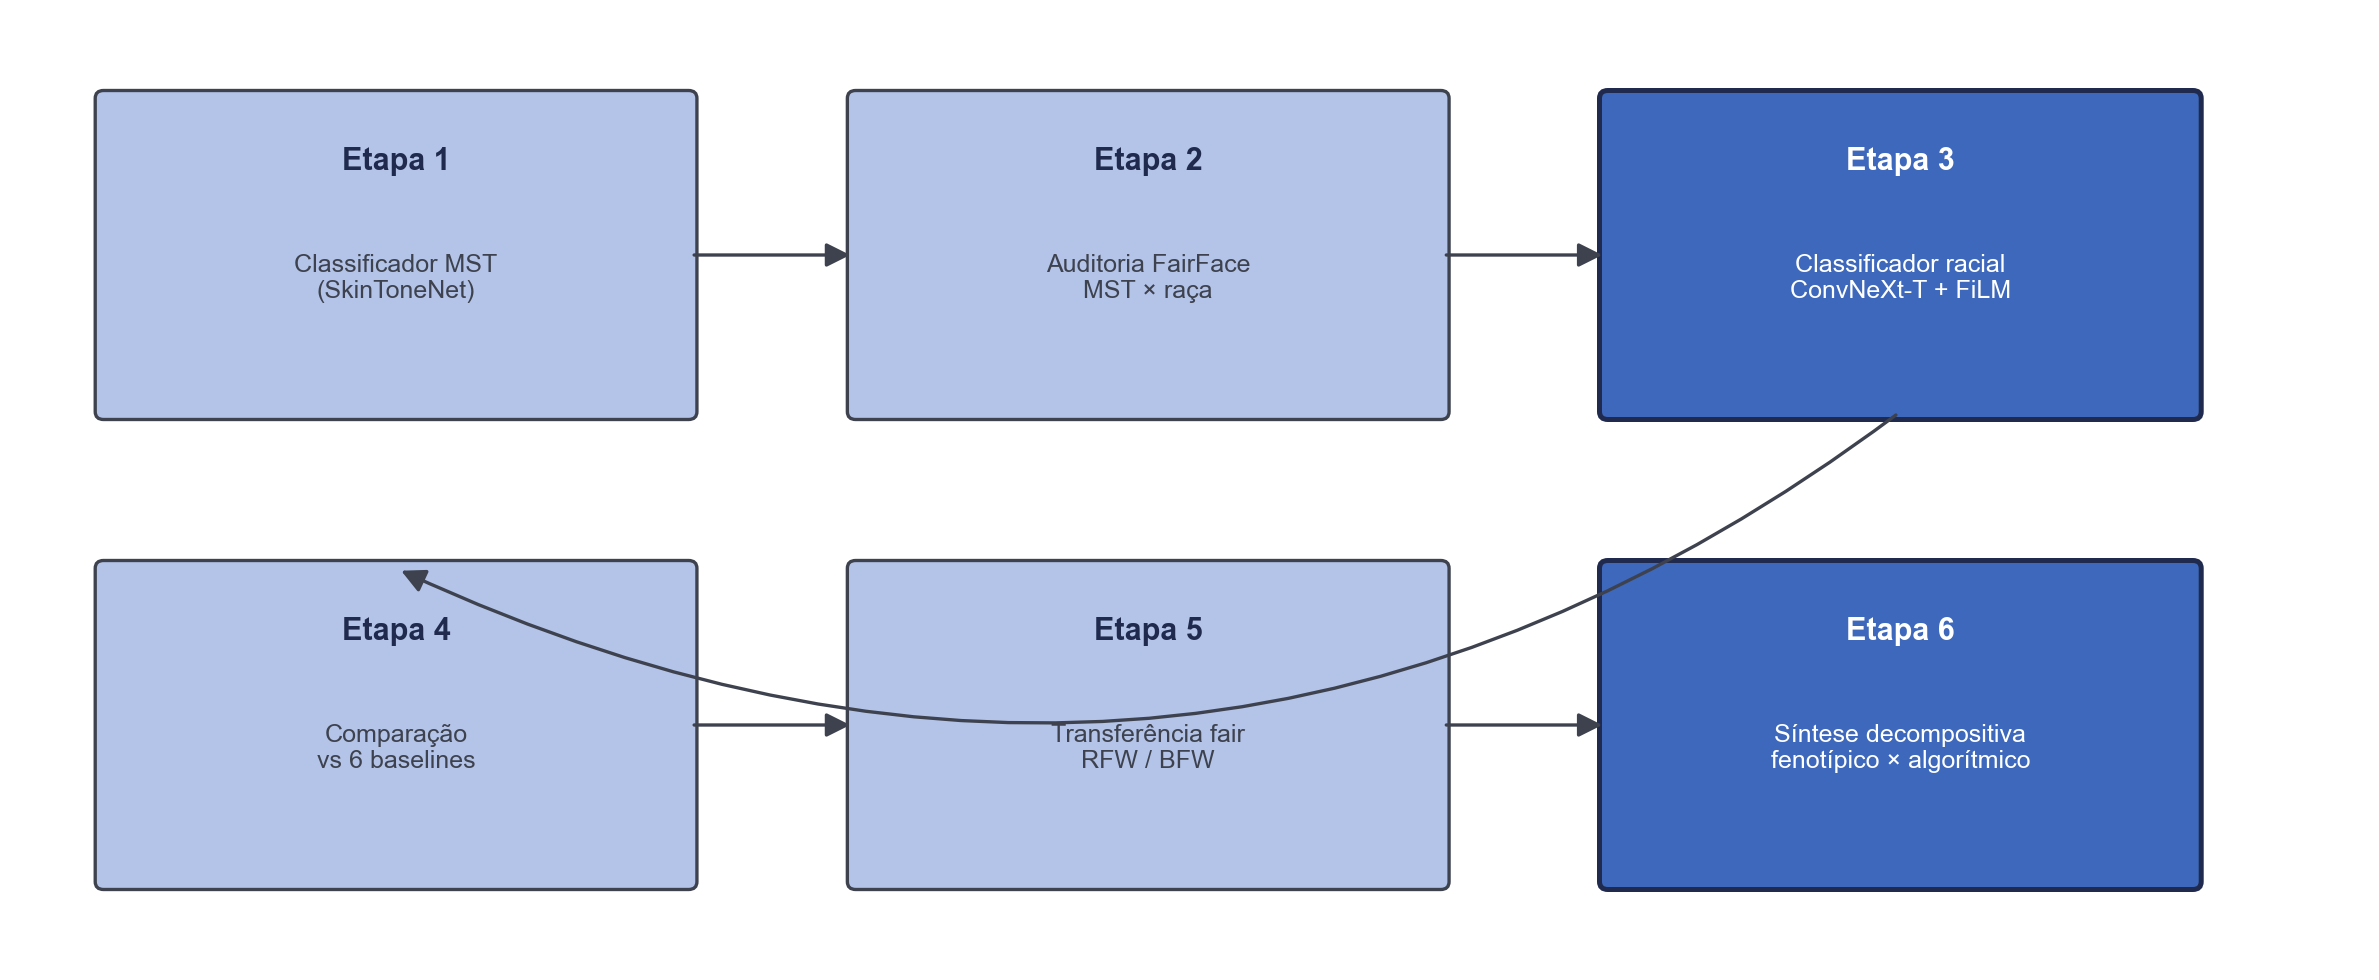
\includegraphics[width=14cm]{images/fig_pipeline_6etapas.png}
\\ \small Fonte: Autoria própria. Etapas em destaque (3 e 6) concentram as contribuições metodológica e diagnóstica principais.
\label{fig:pipeline-6etapas}
\end{figure}


\begin{enumerate}
\item \textbf{Etapa 1 --- Classificador MST}: adoção do SkinToneNet~\cite{matias2026large} como insumo pré-treinado. A modalidade de validação é detalhada na Seção~\ref{sec:validacao_interna}.

\item \textbf{Etapa 2 --- Auditoria fenotípica do FairFace}: aplicação do SkinToneNet sobre o FairFace \emph{validation set} e construção da matriz pública Monk Skin Tone~$\times$~classes raciais.

\item \textbf{Etapa 3 --- Classificador racial com \emph{conditioning}}: treinamento de ConvNeXt-T \emph{fine-tuned} em FairFace \emph{train}, com camadas FiLM~\cite{perez2018film} por estágio recebendo como contexto o vetor MST produzido na Etapa~1.

\item \textbf{Etapa 4 --- Comparação contra \emph{baselines}}: avaliação sistemática do pipeline contra seis \emph{baselines} de mitigação (Seção~\ref{sec:baselines}), com triangulação completa de métricas (Seção~\ref{sec:metricas}).

\item \textbf{Etapa 5 --- Transferência \emph{fair}}: aplicação do \emph{backbone} \emph{fair-trained} para tarefa \emph{downstream} de \emph{face recognition} nos datasets RFW~\cite{wang2019racial} e/ou BFW~\cite{robinson2020face}, com controle explícito de \emph{pixel information} (fração de pixels úteis da face obtida por segmentação BiSeNet) como \emph{confounder} principal, conforme metodologia proposta por \citeonline{pangelinan2023exploring}. Como salvaguarda adicional, estratificam-se os resultados por três descritores complementares de qualidade de imagem --- luminância média (canal $L^*$ da escala CIELAB), nitidez (variância do Laplaciano) e resolução efetiva da face em pixels ---, permitindo verificar se a disparidade residual persiste após controle desses fatores ópticos e blindando a Etapa~6 contra a crítica de que o erro Latinx seria puramente sensorial em vez de fenotípico.

\item \textbf{Etapa 6 --- Síntese decompositiva}: combinação dos resultados obtidos nas Etapas~2 e~5 para quantificar a contribuição relativa do componente fenotípico (irredutível, associado ao \emph{overlap} MST intra-categoria) \emph{versus} componente algorítmico (mitigável) do erro de classificação Latinx.
\end{enumerate}

\section{Datasets utilizados}
\label{sec:datasets}

Todos os datasets adotados são secundários e publicamente disponíveis, sem coleta primária associada:

\begin{description}[font=\bfseries\sffamily]
\item[Treino de classificação racial]: FairFace \emph{train split}, 86.744 imagens com sete classes raciais~\cite{karkkainen2021fairface}.
\item[Validação de MST]: STW~\cite{matias2026large} e Casual Conversations v2~\cite{porgali2023casual}.
\item[Teste de classificação racial]: FairFace \emph{test split}, 10.954 imagens~\cite{karkkainen2021fairface}.
\item[Teste de transferência \emph{fair}]: RFW~\cite{wang2019racial} e/ou BFW~\cite{robinson2020face}.
\end{description}

\section{Baselines de comparação}
\label{sec:baselines}

Seis \emph{baselines} de mitigação algorítmica compõem o quadro comparativo, escolhidos para cobrir cinco famílias metodológicas distintas --- linha canônica, controle arquitetural moderno, aprendizado contrastivo, otimização robusta a distribuição, atenção multi-camada e \emph{debiasing} adversarial:

\begin{enumerate}
\item ResNet-34, \emph{baseline} canônico originalmente treinado por \citeonline{karkkainen2021fairface} sobre o FairFace~\cite{aldahoul2024exploring};
\item ConvNeXt-T puro, sem \emph{conditioning}, como controle arquitetural moderno;
\item FSCL+~\cite{park2022fair};
\item Group DRO~\cite{sagawa2020distribution};
\item FineFACE~\cite{manzoor2024fineface};
\item \emph{Adversarial debiasing}~\cite{zhang2018mitigating}.
\end{enumerate}

\section{Escolha do \emph{backbone}}
\label{sec:backbone}

O \emph{backbone} adotado é o ConvNeXt-T (variante \emph{Tiny}, aproximadamente 28 milhões de parâmetros), da família ConvNeXt proposta como sucessora arquitetural moderna da linha ResNet. A escolha deste \emph{backbone}, em detrimento de outras arquiteturas modernas de igual ou menor porte, fundamenta-se em quatro critérios objetivos:

\begin{enumerate}
\item \textbf{Paridade competitiva com Vision Transformers a custo convolucional.} A família ConvNeXt demonstrou, em ImageNet-1K, desempenho comparável a Swin Transformers com custo de inferência inferior, mantendo a estrutura hierárquica em quatro estágios característica de ResNets, o que permite reaproveitamento imediato de mecanismos de \emph{conditioning} projetados originalmente para redes convolucionais como o FiLM.
\item \textbf{Estabilidade de treinamento em \emph{fine-tuning}.} O uso de \emph{LayerNorm} no lugar de \emph{BatchNorm} confere robustez a variações de \emph{batch size}, comportamento relevante em cenários de treinamento com múltiplas configurações e três sementes independentes (Seção~\ref{sec:rigor}).
\item \textbf{Compatibilidade com o mecanismo FiLM.} A estrutura hierárquica em quatro estágios do ConvNeXt-T oferece pontos de inserção naturais para camadas FiLM logo após cada bloco convolucional principal, sem exigir modificação de \emph{depthwise convolutions} ou de \emph{inverted bottleneck blocks}.
\item \textbf{Comparabilidade com o \emph{baseline} canônico da literatura de \emph{fairness} facial.} A adoção do ConvNeXt-T como controle arquitetural moderno (Configuração A, Seção~\ref{sec:ablation}) permite isolar o efeito do \emph{conditioning} sem confundi-lo com ganhos derivados apenas da modernização do \emph{backbone} sobre o ResNet-34 usado por \citeonline{karkkainen2021fairface}.
\end{enumerate}

Como \emph{sanity check} arquitetural, o trabalho reporta explicitamente o desempenho do ConvNeXt-T puro (Configuração A) em separado do desempenho do ConvNeXt-T com FiLM (Configuração B), permitindo à banca examinadora avaliar de forma independente a contribuição do \emph{backbone} e a contribuição do mecanismo de \emph{conditioning}.

\section{Mecanismo FiLM}
\label{sec:film}

\subsection{Formulação matemática}

Para cada um dos quatro estágios hierárquicos do \emph{backbone} ConvNeXt-T, insere-se uma camada FiLM~\cite{perez2018film} imediatamente após o bloco convolucional principal do estágio. A camada recebe como sinal condicionante o vetor $z \in \mathbb{R}^{10}$ correspondente à saída \emph{softmax} do SkinToneNet pré-treinado~\cite{matias2026large}, e produz parâmetros de modulação $(\gamma_i, \beta_i) \in \mathbb{R}^{C_i} \times \mathbb{R}^{C_i}$ por canal, onde $C_i$ é o número de canais da \emph{feature map} intermediária do estágio $i$. A modulação é aplicada como transformação afim canal a canal:

\begin{equation}
\mathrm{FiLM}(F_i \mid \gamma_i, \beta_i) = \gamma_i \odot F_i + \beta_i,
\qquad
\gamma_i = f_\gamma(z), \quad \beta_i = f_\beta(z),
\label{eq:film}
\end{equation}

onde $F_i \in \mathbb{R}^{H_i \times W_i \times C_i}$ é a \emph{feature map} intermediária do estágio $i$ e $\odot$ denota multiplicação elemento a elemento com \emph{broadcast} nas dimensões espaciais $H_i \times W_i$. Segue-se rigorosamente a formulação original de FiLM~\cite{perez2018film}, sem alterações estruturais no bloco de modulação.

\subsection{Implementação de $f_\gamma$ e $f_\beta$}

As funções $f_\gamma$ e $f_\beta$ são implementadas por duas \emph{Multi-Layer Perceptrons} independentes com arquitetura de duas camadas ($\mathbb{R}^{10} \to \mathbb{R}^{128} \to \mathbb{R}^{C_i}$) e ativação intermediária ReLU. A camada final é inicializada de forma a produzir $\gamma_i \approx 1$ e $\beta_i \approx 0$ no início do treinamento (transformação identidade), garantindo que o modelo inicie o treinamento operando efetivamente como o \emph{backbone} sem \emph{conditioning}, estratégia consistente com práticas de estabilidade de treinamento em mecanismos aditivos residuais~\cite{perez2018film}.

Considerando os quatro estágios do ConvNeXt-T com $C_i \in \{96, 192, 384, 768\}$, o \emph{overhead} paramétrico agregado é de aproximadamente 380.000 parâmetros adicionais, o que corresponde a cerca de 1{,}3\,\% do total de parâmetros do \emph{backbone} (28 milhões). Este \emph{overhead} é substancialmente inferior a alternativas como \emph{cross-attention} (aproximadamente 3\,$\times$ o custo) e mesmo a \emph{Conditional Batch Normalization} implementada com MLPs de mesma capacidade, mantendo a compatibilidade computacional com \emph{fine-tuning} em GPUs de porte comum (Seção~\ref{sec:riscos}, Risco~4).

\subsection{Racional da escolha}

A escolha de FiLM sobre alternativas de \emph{conditioning} é justificada pela combinação de eficiência paramétrica, capacidade demonstrada de modulação por escala e deslocamento em nível de canal e histórico de sucesso em \emph{Visual Question Answering}~\cite{perez2018film}. A análise comparativa completa contra sete alternativas (\emph{Concatenação}, \emph{Conditional Batch Normalization}, \emph{Cross-attention}, AdaIN, SPADE, \emph{HyperNetworks}, LoRA/Adaptadores) é apresentada na Seção~\ref{sec:rl_conditioning_alt} da Revisão Bibliográfica, e a limitação de linearidade do FiLM padrão é endereçada empiricamente pela Configuração~C (FiLM com porta multiplicativa) do estudo de \emph{ablation} (Seção~\ref{sec:ablation}).

A Figura~\ref{fig:mecanismo-film} ilustra a integração do mecanismo FiLM à arquitetura ConvNeXt-T proposta, evidenciando os pontos de inserção da camada de modulação por estágio.

\begin{figure}[htbp]
    \centering
    \caption{Integração do mecanismo FiLM à arquitetura ConvNeXt-T.}
    \centering
    
\includegraphics[width=14cm]{images/film_pipeline.png}
    \\ \small Fonte: Autoria própria.
    \label{fig:mecanismo-film}
\end{figure}

\subsection{Detalhes de treinamento}

Todos os experimentos das quatro configurações (Seção~\ref{sec:ablation}) são conduzidos sob protocolo unificado:

\begin{itemize}
\item \textbf{Otimizador}: AdamW com \emph{learning rate} $1 \times 10^{-4}$ para o \emph{backbone} e $1 \times 10^{-3}$ para as camadas FiLM, \emph{weight decay} de $0{,}05$.
\item \textbf{Escalonamento}: \emph{cosine annealing} com \emph{warmup} linear nos primeiros 5\,\% dos passos.
\item \textbf{\emph{Batch size}}: 64 imagens de $224 \times 224$ pixels.
\item \textbf{Regularização}: \emph{dropout} $0{,}1$ nas MLPs de $f_\gamma$ e $f_\beta$; augmentação padrão (flip horizontal, \emph{color jitter} moderado).
\item \textbf{Critério de parada}: \emph{early stopping} baseado em F1 macro no \emph{validation set} com paciência de 5 épocas.
\item \textbf{\emph{Framework}}: PyTorch 2.x sobre implementação de referência de ConvNeXt disponível em \emph{TorchVision}, com camadas FiLM implementadas como \emph{PyTorch modules} customizados.
\end{itemize}

Estes hiperparâmetros são fixados a priori e mantidos idênticos entre as quatro configurações (A, B, C, D) descritos na Seção~\ref{sec:ablation} e entre os seis \emph{baselines} (Seção~\ref{sec:baselines}), garantindo que diferenças de desempenho observadas sejam atribuíveis exclusivamente à variação do mecanismo de \emph{conditioning} ou da arquitetura do \emph{baseline}, e não a diferenças de otimização.


\section{\emph{Ablation} arquitetural}
\label{sec:ablation}

Este pesquisa conduzirá \emph{ablation} arquitetural comparando quatro configurações do estágio de \emph{conditioning}, mantidos idênticos o \emph{backbone} (ConvNeXt-T), o dataset (FairFace) e o protocolo de avaliação:

\begin{description}[font=\bfseries\sffamily]
\item[Configuração A --- Baseline sem \emph{conditioning}]: ConvNeXt-T \emph{fine-tuned} sem qualquer sinal auxiliar, como controle.
\item[Configuração B --- FiLM linear com MST 10-dim]: proposta principal do trabalho, com $f_\gamma$ e $f_\beta$ implementadas por \emph{Multi-Layer Perceptrons} lineares. Corresponde ao teste da hipótese central de que o \emph{conditioning} arquitetural por tom de pele reduz a disparidade demográfica sem sacrificar acurácia agregada.
\item[Configuração C --- FiLM com porta multiplicativa (\emph{gating} sigmoide)]: variante não-linear proposta como \emph{ablation} nesta pesquisa, inspirada na formulação de mecanismos de \emph{gating} como caso restrito de FiLM discutida por \citeonline{dumoulin2018featurewise}, aplicada para isolar o efeito da linearidade das funções de modulação.
\item[Configuração D --- FiLM sobre \emph{embedding} CLIP-\emph{text} 512-dim]: alternativa moderna, com sinal condicionante em \emph{embedding} semântico produzido por CLIP-\emph{text}~\cite{luo2024fairclip} em vez do vetor MST discreto. O \emph{prompt} adotado é a média de \emph{embeddings} de dez \emph{templates} equivalentes na forma \emph{``a photo of a person with Monk Skin Tone $k$''}, com $k \in \{1, \ldots, 10\}$, ponderados pela probabilidade \emph{softmax} de cada classe MST produzida pelo SkinToneNet. Esta estratégia de \emph{prompt ensembling}, alinhada às práticas de \citeonline{dehdashtian2024fairerclip}, evita a sensibilidade do CLIP a formulações isoladas e produz sinal condicionante mais robusto que \emph{prompts} estáticos únicos.
\end{description}

A Figura~\ref{fig:configuracoes-abcd} compara visualmente as quatro configurações, evidenciando as dimensões variadas (mecanismo de \emph{conditioning} e sinal condicionante) e as dimensões controladas (\emph{backbone}, dataset, protocolo de avaliação).

\begin{figure}[htbp]
\centering
\caption{Quatro configurações comparativas do estudo de \emph{ablation} arquitetural.}
\centering
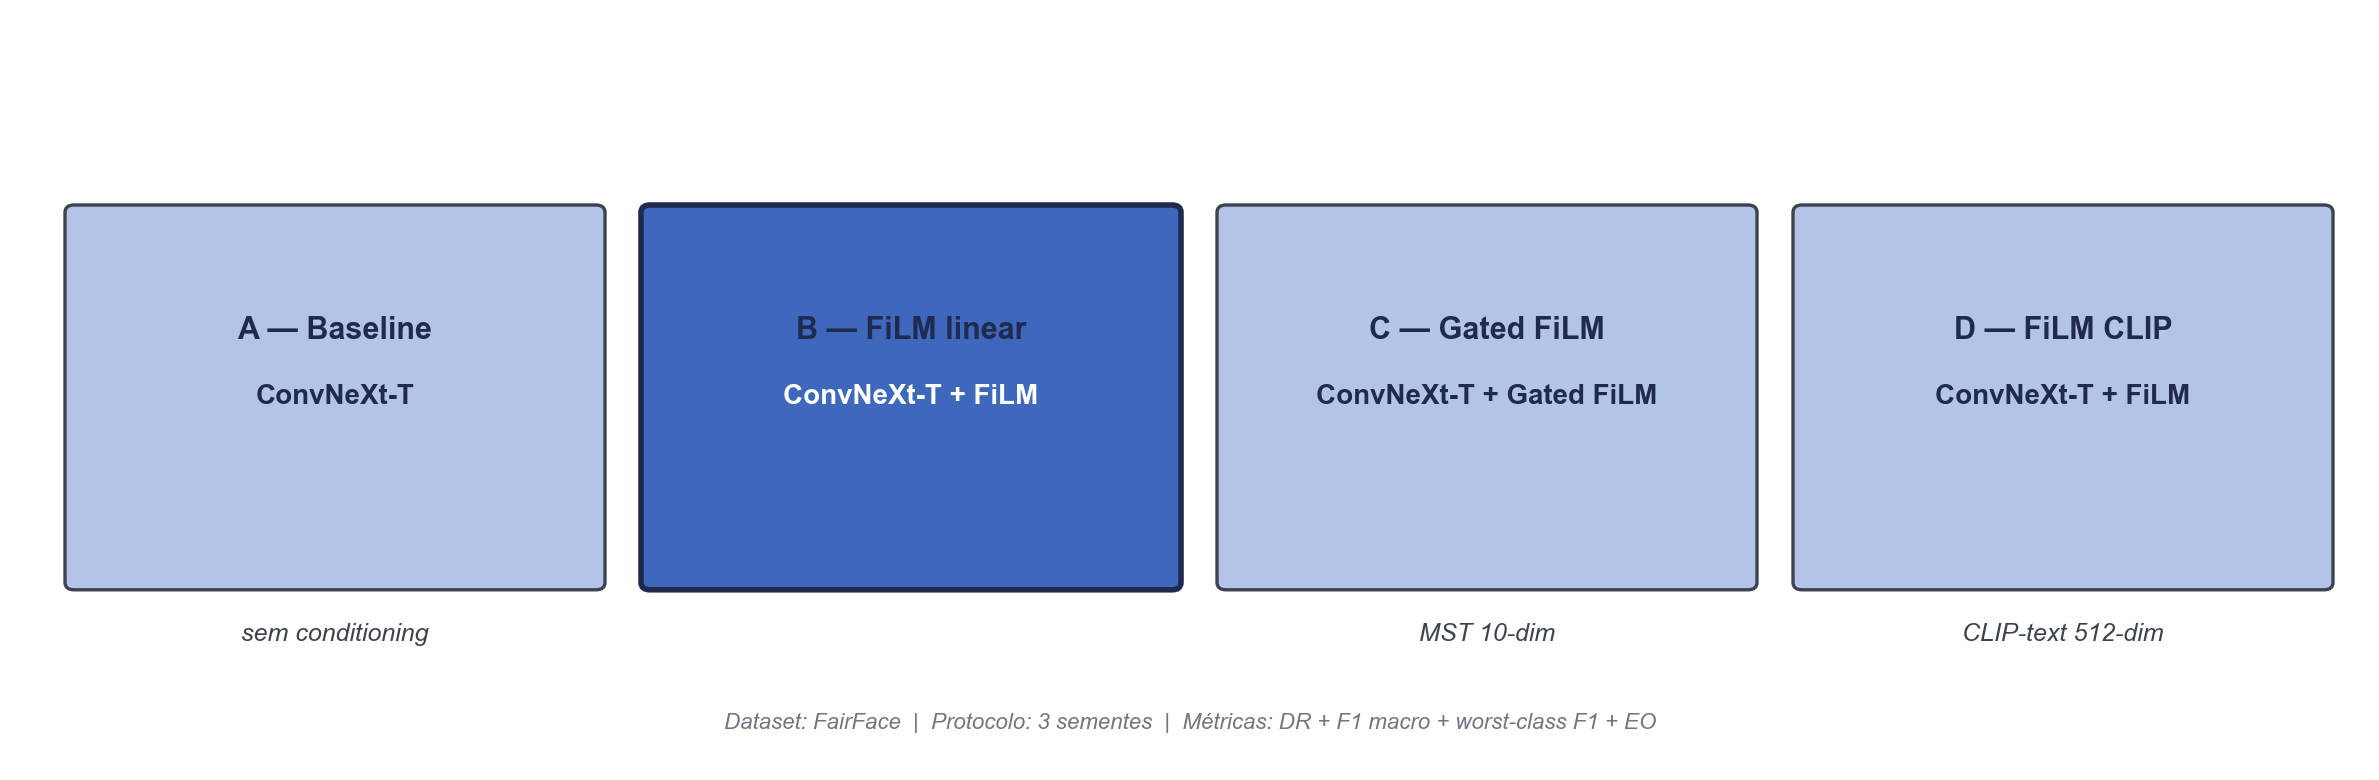
\includegraphics[width=14cm]{images/fig_configs_abcd.png}
\\ \small Fonte: Autoria própria. A Configuração B (proposta principal) é destacada em cor mais intensa.
\label{fig:configuracoes-abcd}
\end{figure}

\section{Triangulação de métricas}
\label{sec:metricas}

Fundamentada no Teorema da Impossibilidade~\cite{kleinberg2017inherent}, que estabelece a impossibilidade de satisfazer simultaneamente múltiplas definições formais de \emph{fairness}, a avaliação é conduzida em dois cenários complementares.

O \textbf{Cenário A} concentra-se no atributo sensível principal desta pesquisa (raça) e adota métricas adequadas ao regime \emph{multi-classe} de sete categorias do FairFace. O \textbf{Cenário B} incorpora a dimensão de gênero apenas como \emph{análise interseccional} de robustez, sem alterar o foco declarado no viés racial, por três razões metodológicas: (i) o estudo seminal \emph{Gender Shades} de \citeonline{buolamwini2018gender} estabeleceu a análise conjunta \emph{race}~$\times$~\emph{gender} como padrão auditável no campo, e a omissão dessa dimensão configuraria retrocesso metodológico em relação ao estado da arte; (ii) o dataset BFW~\cite{robinson2020face}, adotado na Etapa~5 de transferência \emph{fair}, é construído explicitamente sobre oito subgrupos formados pelo cruzamento das duas dimensões, e reportar apenas raça sub-utilizaria o desenho amostral do próprio benchmark; (iii) as definições formais de \emph{Equal Opportunity} e \emph{Equalized Odds} de \citeonline{hardt2016equality} são naturalmente binárias, o que torna sua aplicação sobre o eixo binário de gênero uma correspondência direta, ao passo que a extensão \emph{multi-classe} sobre raça permanece fragmentada na literatura (Lacuna~G5, Seção~\ref{sec:rl_gaps}). O Cenário B opera, portanto, como \emph{cross-check} contra a hipótese de \emph{hiding bias}: um modelo que apresenta paridade em raça pode ocultar disparidade intra-racial entre gêneros, cenário que só a análise interseccional revelaria.

O protocolo de reporte estratificado adotado nos dois cenários segue as diretrizes da norma internacional \textbf{ISO/IEC 19795-10:2024}~\cite{iso2024biometric}, que estabelece o padrão contemporâneo para quantificação e reporte de variação de desempenho biométrico entre grupos demográficos, convergindo com as obrigações de auditoria de \emph{fairness} previstas no \emph{European AI Act} para sistemas classificados como de alto risco.

\subsection{Cenário A --- \emph{race} apenas}
\begin{itemize}
\item F1 macro, agregada e por classe;
\item \emph{Disparity Ratio}: $\mathrm{DR} = \min_c \mathrm{F1}_c / \max_c \mathrm{F1}_c$;
\item \emph{Worst-class} F1, seguindo o princípio de \emph{Distributionally Robust Optimization}~\cite{sagawa2020distribution}.
\end{itemize}

\subsection{Cenário B --- \emph{race} $\times$ \emph{gender}}
\begin{itemize}
\item \emph{Equal Opportunity} por classe: para cada raça $c$, \emph{gap} entre $\mathrm{TPR}_c^{M}$ e $\mathrm{TPR}_c^{F}$~\cite{hardt2016equality};
\item \emph{Equalized Odds} por classe: \emph{gap} simultâneo em TPR (\emph{true positive rate}) e FPR (\emph{false positive rate})~\cite{hardt2016equality}.
\end{itemize}

\subsection{Visualização Pareto-eficiente}
\label{sec:pareto}

Complementando a triangulação, os resultados das quatro configurações (Seção~\ref{sec:ablation}) e dos seis \emph{baselines} (Seção~\ref{sec:baselines}) são projetados no plano \emph{acurácia $\times$ fairness} para diagnóstico visual de dominância Pareto. Cada modelo é representado por um ponto de coordenadas $(1 - \mathrm{F1_{macro}},\; 1 - \mathrm{DR})$, correspondendo respectivamente a erro agregado e disparidade entre grupos. Uma configuração é dita \textbf{Pareto-superior} quando reduz simultaneamente ambas as coordenadas em relação a outra --- isto é, melhora \emph{fairness} sem degradar utilidade, ou vice-versa. A projeção conjunta permite responder de forma inequívoca se o \emph{conditioning} FiLM sobre MST domina os \emph{baselines} de mitigação ou se opera em um trade-off, alinhando-se à recomendação metodológica de \citeonline{manzoor2024fineface} e \citeonline{dominguezcatena2024dsap} de reportar sistemas de \emph{fairness} sob a lente de fronteira de Pareto.

\section{Validação humana interna}
\label{sec:validacao_interna}

A validação de concordância entre o SkinToneNet e a rotulagem humana, prevista no Objetivo 1, é realizada \textbf{exclusivamente pela equipe acadêmica do projeto} --- Mestrando e Orientador ---, sobre um subset estratificado de aproximadamente duzentas a trezentas imagens do FairFace, com estratificação por raça e por tom MST. Não haverá contratação de anotadores externos nem uso de plataformas de \emph{crowdsourcing}. As métricas de concordância adotadas são o coeficiente $\kappa$ de Cohen \emph{par a par} e a exatidão categórica com intervalo de confiança de 95\,\% obtido por \emph{bootstrap}. A escala reduzida é declarada explicitamente como limitação metodológica, sendo compensada por estratificação rigorosa e por replicação da avaliação com dois ou três classificadores MST alternativos.

\section{Rigor experimental}
\label{sec:rigor}

Todos os experimentos são conduzidos sob os seguintes protocolos de rigor:

\begin{itemize}
\item Três sementes aleatórias independentes (42, 1, 2), com reporte de média e desvio padrão para cada métrica;
\item Comparação pareada casada entre configurações, com o mesmo \emph{split} de dados e a mesma inicialização por semente;
\item Intervalos de confiança de 95\,\% obtidos por \emph{bootstrap} não paramétrico;
\item Reporte estratificado por raça e por interseção raça~$\times$~gênero.
\end{itemize}